\newcommand{\ypred}{y_{pred}}
\newcommand{\ytrue}{y_{true}}

In the following section, we compare the results of the Bayesian method with other classifiers.

\begin{figure}
	\begin{tabularx}{\textwidth}{>{\bfseries}X c c c c c c}
		\toprule
		\textbf{Classifier} & \textbf{Accuracy} & \textbf{Precision} & \textbf{Recall} & \textbf{AUC} & \textbf{$F_1$}-\textbf{score} & \textbf{$F_4$}-\textbf{score} \\
		\midrule
		Método Bayesiano & 0 & 0 & 0 & 0 & 0 & 0 \\
		\midrule
		Random Selection & 0.500 & 0.510 & 0.501 & 0.500 & 0.529 & 0.504 \\
		Majority Voting & 0 & 0 & 0 & 0 & 0 & 0 \\
		\midrule
		Naïve Bayes & 0.569 & 0.550 & 0.711 & 0.550 & 0.649 & 0.703 \\
		K Nearest Neighbors\footnote{Selecting $K = 9$} & 0.551 & 0.589 & 0.666 & 0.55 & 0.625 & 0.661 \\
		SVM with RBF kernel\footnote{Selecting $C = 100$} & 0.559 & 0.561 & 0.947 & 0.571 & 0.705 & 0.910 \\
		Logistic Regression\footnote{Selecting $C = 0.01$} & 0.563 & 0.563 & 0.991 & 0.569 & 0.718 & 0.949 \\
		Stochastic Gradient Descent & 0.557 & 0.575 & 0.861 & 0.516 & 0.679 & 0.833 \\
		Random Forest & 0.570 & 0.571 & 0.638 & 0.668 & 0.606 & 0.673 \\
		\midrule
		Categorized LR & 0 & 0 & 0 & 0 & 0 & 0 \\
		Count Link Model & 0 & 0 & 0 & 0 & 0 & 0 \\
		\bottomrule
	\end{tabularx}
\end{figure}

\subsection{Random Selection}

For completeness sake we created a random classifier for the socioeconomic category of each user.

We applied two other inference methods to the same data and compared their accuracies to our Bayesian model.

\begin{itemize}
	\item \textbf{Random selection} which chooses randomly the category for each user.
	\item \textbf{Majority voting} which decides whether a user is in the high or low income category depending on the category of the majority of its contacts. In case of a tie, the category is chosen randomly.
\end{itemize}

The \emph{accuracy} of the first method is as expected \num{0.5}, while the \emph{accuracy} for majority voting is \num{0.66}.
With the Bayesian method we obtain an \emph{accuracy} of \num{0.71}.

\subsection{Machine Learning Validation Metrics}

In the following subsections we present the outline of several supervised machine learning algorithms which are used to compare the Bayesian method to a more realistic baseline. First, we'll present several ways to validate the different algorithms when applied to the data. In the following section, we'll present many of the algorithms used for comparison.

Given a set of features $X$ with labels $y$, called \textbf{training data}, and another set of features $Z$ without labels, we want to create an a binary classifier represented as a learning function $g : X \rightarrow y$ that will predict certain values of $y$ that are as close as possible to the real values.

There are many metrics that can be used to measure the performance of a classifier or a predictor~\cite{binaryevaluation}; different fields have different preferences due to different goals. In this section, we present many metrics to evaluate different results that are commonly used in the area of mobile phone data analysis~\cite{oskardottir2016}.

\subsubsection{Classification of individual results}

We can easily see the problem of income predicition with the parameters we presented in~\ref{inference_methodology} as a binary classification task, where each instance represents a person and it's positive when this person is in the upper quantile of wealth $\closeopen{6300}{\infty}$, and negative when it is in the lower quantile $\closeopen{1000}{6300}$.

Once we define out classifier $g$ and run it against a matrix\maybe{Set?} of features\maybe{Should I explain train/test split before this subsubsection?}, we get a predicted result $\ypred$ which, when compared to the actual result $\ytrue = y$, can be classified as the one in table~\ref{confusion}.

\begin{figure}[h]
\begin{tabularx}{\textwidth}{| c | X | X X |}
\hline

& & \multicolumn{2}{c|}{\textbf{Predicted Condition}} \\
& Total Population &
\makecell{Condition Positive} &
\makecell{Condition Negative} \\ \hline

\multirow{2}{5em}{\textbf{True Condition}} &
Condition Positive &
\cellcolor{OrangeRed} \makecell{\textbf{True Positive}} &
\cellcolor{CadetBlue} \makecell{\textbf{False Negative} \\ (Type II error)} \\


& Condition Negative &
\cellcolor{CadetBlue} \makecell{\textbf{False Positive} \\ (Type I Error)} &
\cellcolor{OrangeRed} \makecell{\textbf{True Negative}} \\ \hline

\end{tabularx}
\label{confusion}
\caption[caption]{Confusion Table, showing different classifications of an individual prediction. \\ True and False Positives ($\TP$/$\FP$) refer to the number of predicted positives that were correct/incorrect, and similarly for True and False Negatives ($\TN$/$\FN$).}
\end{figure}

Additionally, this table can be easily seen in a graphical way in figure~\ref{fig:truefalsenegativepositive}.

\begin{figure}
\centering
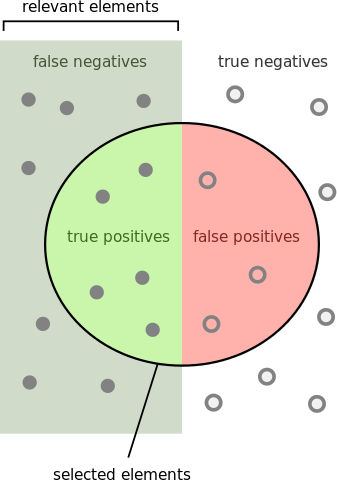
\includegraphics[width=15em]{figures/TrueFalseNegativePositive.png}
\caption{Visual explanation of \emph{Precision} and \emph{Recall}}
\label{fig:truefalsenegativepositive}
\end{figure}

\subsubsection{Precision and Recall} \emph{Precision} denotes the proportion of predicted positive cases that are correctly real positive. Trying to maximize this would allow us to adjust a particular predictor so that the majority of the predicted cases are actually positive. Conversely, \emph{recall} is the proportion of real positive cases that are correctly predicted positive, and maximizing it would allow us to adjust a predictor so that the majority of positive cases are predicted.

\begin{equation}
\begin{split}
\Precision = \TPA &= \frac{\TP}{\TP + \FP} \\
\Recall = \TPR &= \frac{\TP}{\TP + \FN}
\end{split}
\label{precisionrecall}
\end{equation}

These two measures and their combinations focus only on the positive examples and predictions, althrough between them they capture some information about the rates and kind of errors made\cite{binaryevaluation}. While the \emph{recall} has been shown to have a major weight in working with machine translation\cite{fraser2007}, they aren't particularly useful to use alone since they don't take into account many factors of the prediction\cite{binaryevaluation}.

\subsubsection{Inverse~Precision and Inverse~Recall}

As a corollary of the previous metrics, we can add metrics that measure the proportion of real negative cases that are correctly predicted negative, referred as the \emph{Inverse~Recall}, and the proportion of predicted negatives that are real negatives, referreed as the \emph{Inverse~Precision}\cite{binaryevaluation}. We can see that these are equivalent to finding the \emph{Precision} and \emph{Recall} of the negative category.

\begin{equation}
\begin{split}
\InvPrecision = \TNR &= \frac{\TN}{\FP + \TN} \\
\InvRecall = \TNA &= \frac{\TN}{\FN + \TN}
\end{split}
\label{negativeprecisionrecall}
\end{equation}

\subsubsection{Accuracy}

The \emph{accuracy}, commonly referred in te context of binary classifiers as \textbf{Rand~Accuracy}\cite{powers15}, is used as a statistical measure of how well a binary classification test identifies or excludes a condition. Unlike the \emph{precision}, it takes into account the negatives, and it's expressible\cite{binaryevaluation} both as a weighted average of \emph{precision} and inverse \emph{precision} or \emph{recall} and \emph{inverse recall}.

\begin{equation}
\Accuracy = \frac{\TP + \TN}{N}
\label{accuracy}
\end{equation}

This can be more simply expressed using the weighted average of either the \emph{Precision} and \emph{Inverse~Precision} or the \emph{Recall} and the \emph{Inverse~Recall}.

\begin{equation}
\begin{split}
\Accuracy &= \left(\TP + \TN\right) \cdot \TPR + \left(\FP + \TN\right) \cdot \TNR \\
&= \left(\TP + \FP\right) \cdot \TPA + \left(\FN + \TN\right) \cdot \TNA
\end{split}
\label{accuracy2}
\end{equation}

\subsubsection{ROC Curve}

A \emph{Receiver Operating Characteristing} graph is a technique for visualizing, organizing, and selecting classifiers based on their performance\cite{fawcett2005}. The curve is created by plotting the \emph{True Positive Rate} against the \emph{False Positive Rate} at various threshold settings.

This allows to compare different classifiers before having to select a particular threshold value for them. In particular, a random classifier will score near the positive diagonal ($\FPR = \TPR$), while a perfect classifier will score in the top left hand corner ($\FPR = 1, \TPR = 0$) and a worst case classifier will score in the bottom right hand corner\footnote{Note that, for any binary classifier, it's trivial to transpose the entire ROC curve (or a part of it) to the other part of the diagonal; therefore the worst ``realistic'' case is the random one}\cite{binaryevaluation}.

\begin{figure}
\todo{Add figure of ROC with AUC}
\caption{A \emph{ROC Curve}, where the \emph{Area Under the Curve} is marked}
\label{fig:roc}
\end{figure}

\subsubsection{Area Under the Curve}

The \emph{ROC Curve} allows us to compare classifiers and choose the one which is closer to optimal in some sense. While there are many possible parametrizations, the most common is to minimize the \emph{Area Under the Curve}, which is equal to the probability that a classifier will rank a randomly chosen positive instance higher than a randomly chosen negative one\cite{fawcett2005}. This can be formulated as shown in formula~\ref{eq:auc}.

\begin{equation}
\begin{split}
\AUC &= P\left(X_1 > X_0\right) \\
&= \todo{Something something}
\end{split}
\label{eq:auc}
\end{equation}

\subsubsection{F-measure}

The \emph{F-measure} is another measure of a tests accuracy. It considers both the \emph{Precision} and the \emph{Recall} of the test to compute the score. It can be considered the weighted average of both values for some weight $\beta$, where $F_\beta$ reaches the best score 1 when both precision and recall are 1.

\begin{equation}
\begin{split}
F_\beta &= \left( 1 + \beta^2 \right) \cdot \frac{\TPA \cdot \TPR}{\left( \beta^2 \cdot \TPA \right) + \TPR} \\
&= \frac{\left( 1 + \beta^2 \right) \cdot \TP}{\left( 1 + \beta^2 \right) \cdot \TP + \beta^2 \cdot \FN + \FP}
\end{split}
\end{equation}

The most commonly used \emph{F-measure}, $F_1$, measures the \emph{Precision} and \emph{Recall} is thet harmonic mean of the \emph{Precision} and \emph{Recall}. In particular, for an \emph{F-measure} with $\beta > 1$ weights Recall higher than Precision, while with $beta < 1$ weights Precision higher than Recall.

\subsection{Graph Sampling and Categorical User Data}
